\documentclass{article}

\usepackage[spanish]{babel}
\usepackage[margin=1.5in]{geometry}
\usepackage{graphicx}
\usepackage[utf8]{inputenc}

\begin{document}

\setcounter{section}{-1}
\section{Conceptos básicos de redes eléctricas}

\subsection{Conceptos básicos}

\subsubsection{Magnitudes eléctricas}

\begin{itemize}
	\item Intensidad de corriente eléctrica: Cantidad de carga que atraviesa un conductor por unidad de tiempo. Unidad: Ampère / Amperio (A). Órdenes usuales de magnitud (O.U.M.): $\mu$A, mA
	\item Diferencia de potencial (entre dos puntos): Causa/origen del paso de una corriente eléctrica a través
	de un conductor. Unidad: Volt/Voltio (V). O.U.M.: mV, V
	\item Frecuencia: Esta magnitud se verá más en detalle al ver corriente alterna. Unidad: Hertz (Hz).
	 O.U.M.: Hz, kHz, MHz.
\end{itemize}

\subsubsection{Tipos de señales}

Corriente Continua (CC) y Corriente Alterna (CA). En CC, la señal eléctrica se mantiene fija en un valor constante.
En CA, la señal varía de forma senoidal, con cierta amplitud, frecuencia y fase. Cuando estas señales son
generadas por fuentes, se usa la notación de la figura~\ref{fig:001_fuentes}, en la página \pageref{fig:001_fuentes}

\begin{figure}[t]
\caption{Notación circuital para distintos tipos de fuentes}
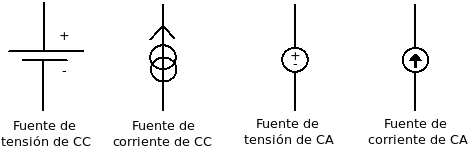
\includegraphics[scale=0.75]{img/teo_fig001_fuentes.png} 
\centering
\label{fig:001_fuentes}
\end{figure}

\subsubsection{Polaridad y sentidos de referencia}

\begin{figure}[t]
\caption{Polaridad y sentidos de referencia en un circuito}
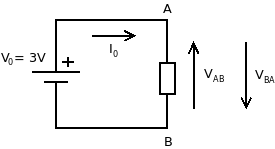
\includegraphics[scale=1]{img/teo_fig002_polaridad.png} 
\centering
\label{fig:002_polaridad}
\end{figure}

Véase la figura ~\ref{fig:002_polaridad}, en la página \pageref{fig:002_polaridad}. La tensión $V_{AB}$ equivale a la diferencia
de potencial $V_A - V_B$, en tanto $V_{BA}$ equivale a $V_B - V_A$. El primer término de la resta, el minuendo, corresponde
a la tensión considerada positiva. Eso es sólo una referencia establecida; puede ser negativa, como se ve en la
figura~\ref{fig:003_voltimetro}, en la página \pageref{fig:003_voltimetro}. Su valor dependerá de las condiciones del
circuito y de cómo se realice la medición.

\begin{figure}[t]
\caption{Polaridad al medir con voltímetro}
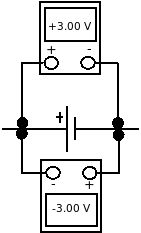
\includegraphics[scale=0.75]{img/teo_fig003_voltimetro.png} 
\centering
\label{fig:003_voltimetro}
\end{figure}

\subsubsection{Masa y tierra}

Por \textbf{masa}, se entiende un punto cuyo potencial se toma como referencia para medir el resto.
En cambio, la \textbf{tierra} es una línea fijada como protección ante posibles descargas.

Corrientes superiores a 1 mA ya son perceptibles si circulan por el cuerpo humano; se dice que 1 mA
es el umbral de percepción. Corrientes mayores a 5 mA ya pueden causar daños a las personas si recorren
su cuerpo.

\begin{figure}[t]
\caption{Conexión a tierra}
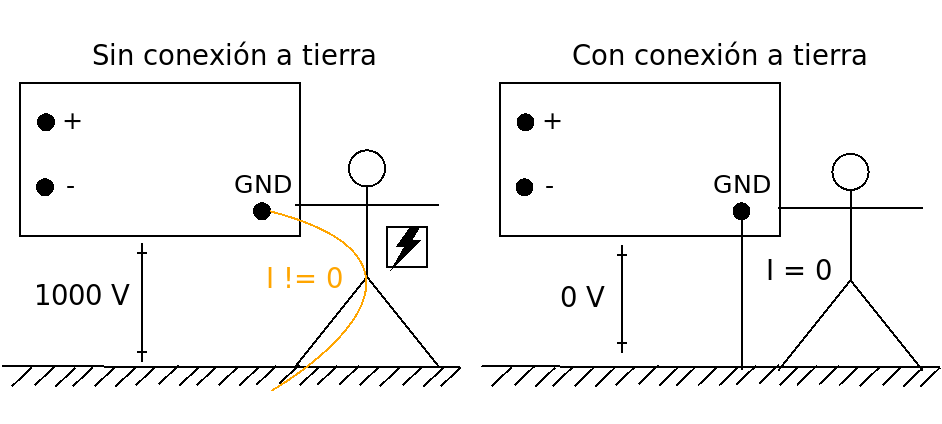
\includegraphics[scale=0.25]{img/teo_fig004_tierra.png} 
\centering
\label{fig:004_tierra}
\end{figure}

\end{document} 